\documentclass[english]{mlutalk}
\usepackage{tikz}
\usepackage{listings}
\usepackage{xspace}
\usepackage{biblatex}
\usepackage{tabularx}
\usepackage{booktabs}
\usepackage{graphicx}
\usepackage{tikz}
\usepackage{tabularx}
\usepackage{multirow}
\usepackage{fontawesome5}
\usepackage{xurl}
\addbibresource{../report/literature.bib}

% Listings
\definecolor{mediumgray}{gray}{0.60}
\definecolor{webiscodebasic}{rgb}{0.2,0.2,0.2}
\definecolor{webiscodekeyword}{rgb}{0.0,0.5,0.0}
\definecolor{webiscodekeywordself}{rgb}{0.7,0.4,0.6}
\definecolor{webiscodeidentifier}{rgb}{0.0,0.0,0.0}
\definecolor{webiscodecomment}{rgb}{0.25,0.5,0.5}
\definecolor{webiscodestring}{rgb}{0.75,0.12,0.12}
\definecolor{webiscodedecorator}{rgb}{0.6,0.3,0.0}
\lstdefinestyle{webisstyle}{
  basicstyle=\ttfamily\footnotesize\color{webiscodebasic},
  keywordstyle=\color{webiscodekeyword},
  identifierstyle=\color{webiscodeidentifier},
  commentstyle=\color{webiscodecomment},
  stringstyle=\color{webiscodestring},
  showstringspaces=false,
  frame=lines,
  framesep=0.7em,
  rulesep=0.5em,
  framerule=0.1em,
  keepspaces=true,
  tabsize=2,
  showtabs=false,
  breakatwhitespace=false,
  breaklines=true,
  prebreak={\mbox{\(\hookleftarrow\)}},
  numbers=none,
  literate=
    {->}{{\textrightarrow}}{2}
    {>=}{{\(\geq\)}}{2}
    {<=}{{\(\leq\)}}{2}
    {!=}{{\(\neq\)}}{2}
    {|>}{{\(\triangleright\)}}{2},
  emptylines=0,
}
\lstloadlanguages{Haskell}
\lstset{
  style=webisstyle,
  language=Haskell,
}

% Editing:
\newcommand{\todocite}{{\smaller\color{red}[CITE]}\xspace}
\newcommand{\todo}[1]{{\smaller\color{red}[#1]}}

% Lists:
\setlength{\itemsep}{2ex}

% Other:
\renewcommand{\emph}[1]{\textbf{#1}}

\title{Insights Towards Safer Roads}
\subtitle{Visualizing Accidents in France from~2005 to~2020}
\author{Jan Heinrich Reimer}
\institute{Martin Luther University Halle-Wittenberg\\Information Retrieval und Visualisierung}
\date{September~14, 2022}
\titlegraphic{
\includegraphics[width=3cm]{figures/mlu-halle}}

\begin{document}

\titleframe

\begin{frame}{Motivation}
  \begin{itemize}
    \item high global number of accidents~\cite{Who2015}
    \item decreasing trend
    \item \emph{1.5\,\%}~of EU citizens report \emph{injuries} from road accidents\footnote{\tiny\url{https://ec.europa.eu/eurostat/databrowser/bookmark/55b45b50-76ac-4cbf-9493-274087bd96fe}}~(in~2009)
    \item \emph{4~out of 100\,000}~inhabitants \emph{die} of road accidents\footnote{\tiny\url{https://ec.europa.eu/eurostat/web/products-eurostat-news/-/DDN-20220511-1}}~(in~2020) \\
    {\scriptsize for comparison: Covid-19 had 0.16~out of~100\,000\footnote{\tiny\url{https://www.eu-info.de/europa/corona/statistik/}}~(up to~06/2021)}
    \item reasons not easy to change:
    \begin{itemize}
      \item inexperience or loss of control~\cite{RolisonRMF2018}
      \item combusted cities~\cite{AlbalateF2021}
      \item insufficient law enforcement~\cite{Who2015}
    \end{itemize}
  \end{itemize}
\end{frame}

\begin{frame}{Target Groups}
  \begin{enumerate}
    \item {\large citizens}
    \begin{itemize}
      \item commuting on roads
      \item no expert knowledge~(e.g., of public infrastructure or mechanical vocabulary)
    \end{itemize}
    \item {\large policymakers}
    \begin{itemize}
      \item governments in Europe
      \item trained~(e.g., law or statistics)
    \end{itemize}
    \item {\large infrastructure planners}
    \begin{itemize}
      \item experts
      \item build new bridges, crossing, etc.
    \end{itemize}
  \end{enumerate}
  \begin{block}{Goal}
    \emph{Where}, \emph{when}, and with \emph{whom} accidents occur most often?
  \end{block}
\end{frame}

\begin{frame}{Application Tasks}
  \begin{block}{Questions}
    \vspace{1ex}
    \footnotesize
    \begin{tabularx}{\linewidth}{lX}
        \toprule
        \textbf{Question} & \textbf{Background} \\
        \midrule
        Are roads more dangerous in winter or summer? & citizen \\
        Do men or women drive more safely? & policymaker \\
        Are there hotspots of accidents in cities or rural areas? & citizen, policymaker \\
        Do dedicated bicycle lanes make roads safer? & citizen, policymaker, infrastructure planner \\
        Are wider roads safer than narrow roads? & citizen, infrastructure planner \\
        \bottomrule
    \end{tabularx}
  \end{block}
  \begin{block}{Mental Models}
    \begin{itemize}
      \item times and dates
      \item geographical position
      \item clustering/categorization
    \end{itemize}
  \end{block}
\end{frame}

\begin{frame}{Dataset}
  \begin{itemize}
    \item French government open data\footnote{\tiny\url{https://data.gouv.fr/en/datasets/bases-de-donnees-annuelles-des-accidents-corporels-de-la-circulation-routiere-annees-de-2005-a-2019/}}
    \item road accidents 2005--2020
    \item 5~CSV files per year:
    \begin{description}[caracteristiques-YYYY.csv]
      \item[caracteristiques-YYYY.csv] characteristics
      \item[lieux-YYYY.csv] location
      \item[usagers-YYYY.csv] persons
      \item[vehicules-YYYY.csv] vehicles
    \end{description}
    \item 64~files from 16~years considered for our visualizations
    \item many nominal dimensions
    \item often incomplete
  \end{itemize}
\end{frame}

\begin{frame}{Preprocessing}
  From this\textellipsis
  \lstinputlisting[linerange={1-3},basicstyle=\fontsize{7pt}{7pt}\ttfamily,language=]{../static/data/cache/caracteristiques-2005.csv}
  and\textellipsis
  \lstinputlisting[linerange={1-3},basicstyle=\fontsize{7pt}{7pt}\ttfamily,language=]{../static/data/cache/usagers-2005.csv}
  \vspace{3ex}
  To this\textellipsis
  \lstinputlisting[linerange={1-1},basicstyle=\fontsize{5.5pt}{5.5pt}\ttfamily,language=Java]{../static/data/accidents-sample.jsonl}
\end{frame}
\begin{frame}{Preprocessing}
  \begin{itemize}
    \setlength{\itemsep}{2ex}
    \item implemented in Python, with Elm's type safety correcting errors in the data is difficult
    \item CSV files different across years
    \begin{itemize}
      \item different separators
      \item different file encodings
      \item fields are named differently
      \item different number formats
    \end{itemize}
    \item group persons by vehicle, vehicles by accident
    \item extract smaller sample~(10\,000 accidents) due to hardware limitations
  \end{itemize}
\end{frame}

\begin{frame}{Visualizations}
  \framesubtitle{Severity Time Series -- Example}
  \begin{figure}
      \centering
      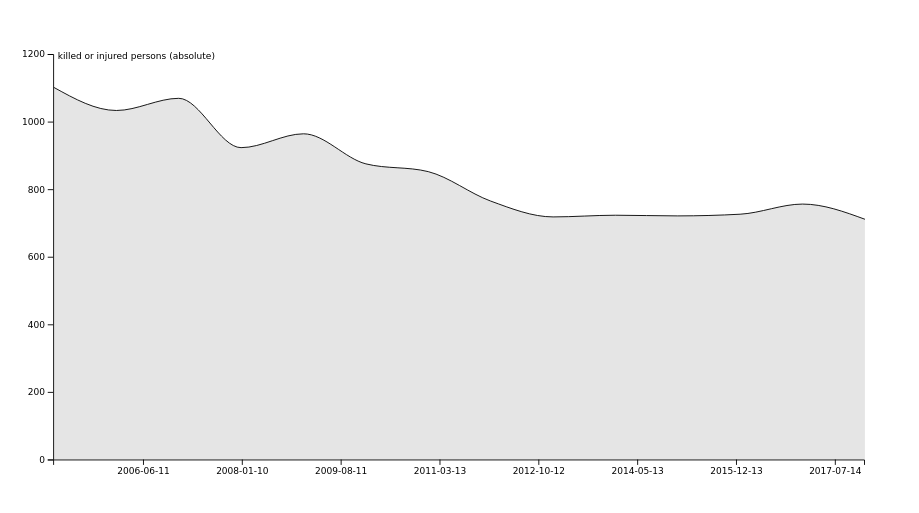
\includegraphics[width=0.8\linewidth]{../report/figures/time-series-2-to-1-killed-or-injured-absolute-never-per-year}
      \vspace*{-3ex}
      \caption{Number of killed or injured persons per year in~2005--2020~(ratio~2:1).}
  \end{figure}
  \vspace*{-2ex}
  \begin{figure}
      \centering
      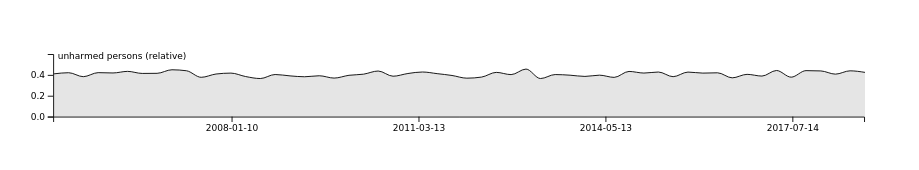
\includegraphics[width=0.8\linewidth]{../report/figures/time-series-banking-45-unharmed-relative-never-per-quarter}
      \vspace*{-3ex}
      \caption{Proportion of unharmed persons in accidents per quarter~(banking to~45\(^\circ\)).}
  \end{figure}
\end{frame}

\begin{frame}{Visualizations}
  \framesubtitle{Severity Time Series}
  \begin{itemize}
    \setlength{\itemsep}{3ex}
    \item aggregate accidents across years~(seasonal patterns)
    \item group per week, month, or year
    \item count killed, injured, killed and injured, unharmed persons
    \item absolute number or relative proportion of persons
    \item manual aspect ratio or banking to~45\(^\circ\)
  \end{itemize}
\end{frame}

\begin{frame}{Visualizations}
  \framesubtitle{Persons Map with Stick Figures -- Example}
  \begin{minipage}{0.49\linewidth}
    \begin{figure}
      \centering
      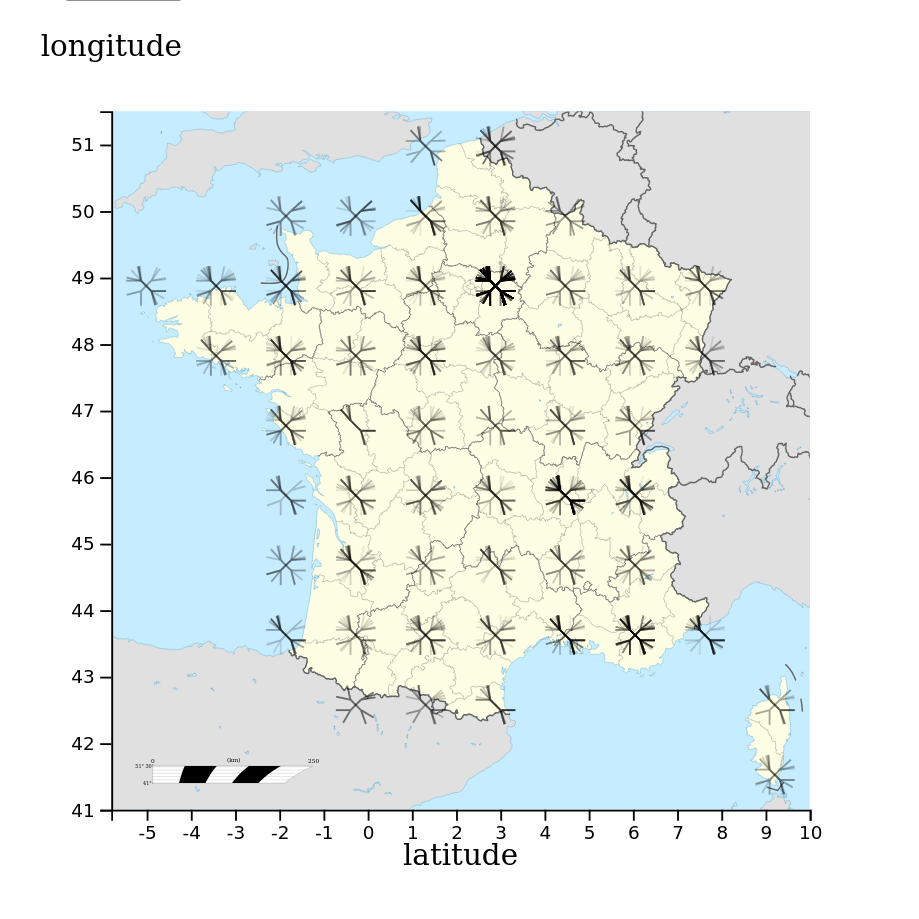
\includegraphics[width=1\linewidth]{../report/figures/stick-figures-by-grid-10-10-xray}
      \caption{Stick figures of persons by \(10 \times 10\)~grid in x-ray style.}
    \end{figure}
  \end{minipage}
  \begin{minipage}{0.49\linewidth}
    \begin{figure}
      \centering
      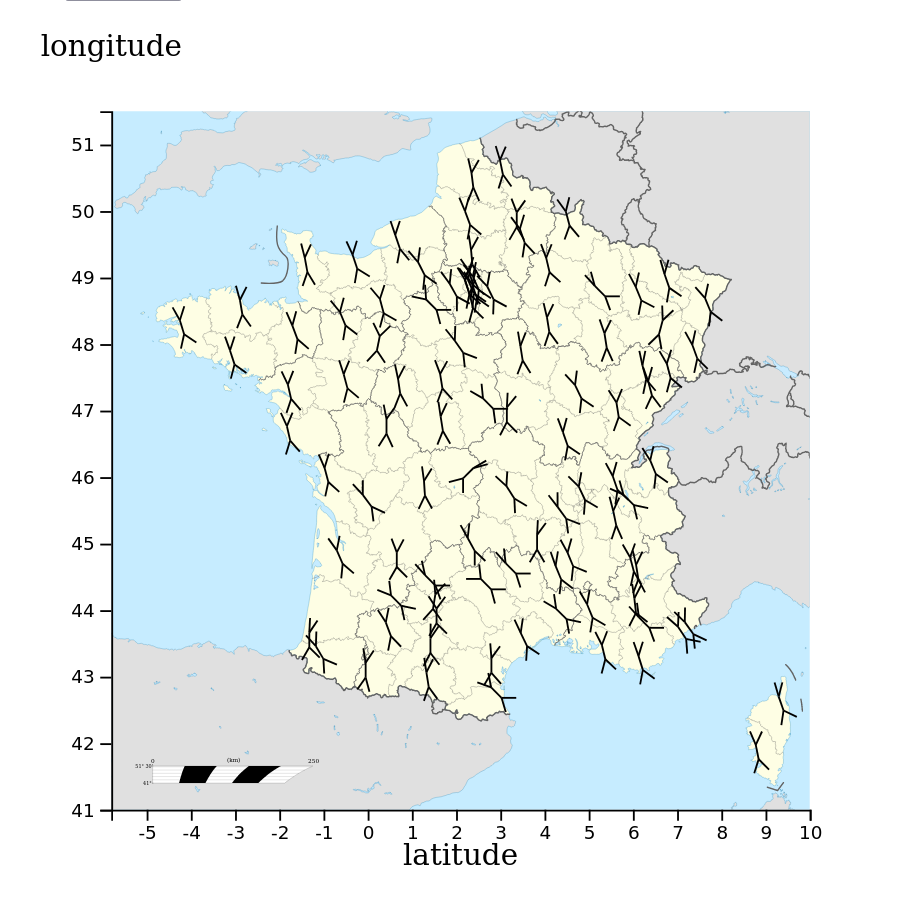
\includegraphics[width=1\linewidth]{../report/figures/stick-figures-by-department-average}
      \caption{Stick figures of average persons by France's Departements.}
    \end{figure}
  \end{minipage}
\end{frame}

\begin{frame}{Visualizations}
  \framesubtitle{Persons Map with Stick Figures}
  \begin{itemize}
    \item stick figure icons~\cite{PickettG1988} of person groups
    \item on geographical map of France\footnote{\tiny\url{https://commons.wikimedia.org/wiki/File:France_location_map-Regions_and_departements-2016.svg}}
    \item display one average stick figure per group
    \item or display each person within a group in x-ray decreasing
    \item group by political body or grid
  \end{itemize}

  \begin{block}{Dimensions}
    \scriptsize
    \begin{description}
      \setlength{\itemsep}{1pt}
      \item[\(\alpha\)] sex, \(-45^\circ\)~(female) or \(45^\circ\)~(male)
      \item[\(\beta\)] birth year, inverted, map to  \([105^\circ; 135^\circ]\)
      \item[\(\gamma\)] travel reason, ordered~(professional, home\(\to\)work, home\(\to\)school, shopping, leisure), map to  \([105^\circ; 135^\circ]\)
      \item[\(\delta\)] safety equipment count, inverted, map to  \([105^\circ; 135^\circ]\)
      \item[\(\epsilon\)] number of persons in vehicle, inverted, map to  \([105^\circ; 135^\circ]\)
    \end{description}
  \end{block}
\end{frame}

\begin{frame}{Visualizations}
  \framesubtitle{Accident Type Treemap -- Example}
  \begin{minipage}{0.49\linewidth}
    \begin{figure}
      \centering
      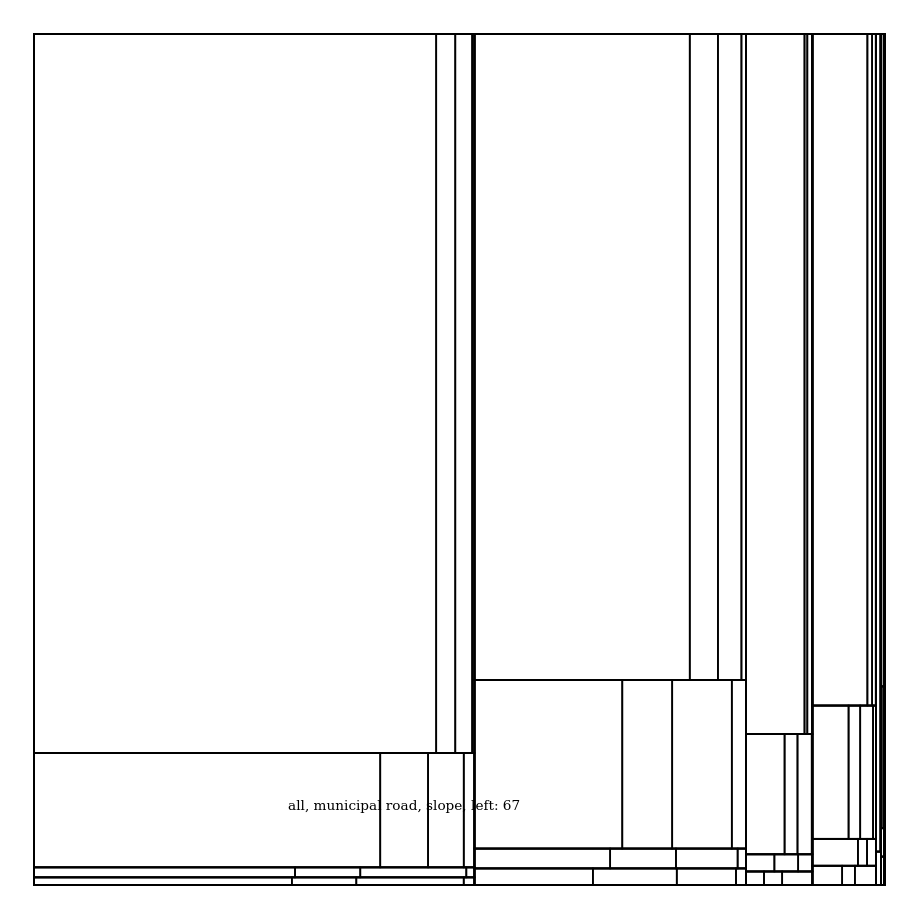
\includegraphics[width=1\linewidth]{../report/figures/tree-treemap-road-category-road-profile-road-curvature}
      \caption{Accidents by road category, profile, curvature.}
    \end{figure}
  \end{minipage}
  \begin{minipage}{0.49\linewidth}
    \begin{figure}
      \centering
      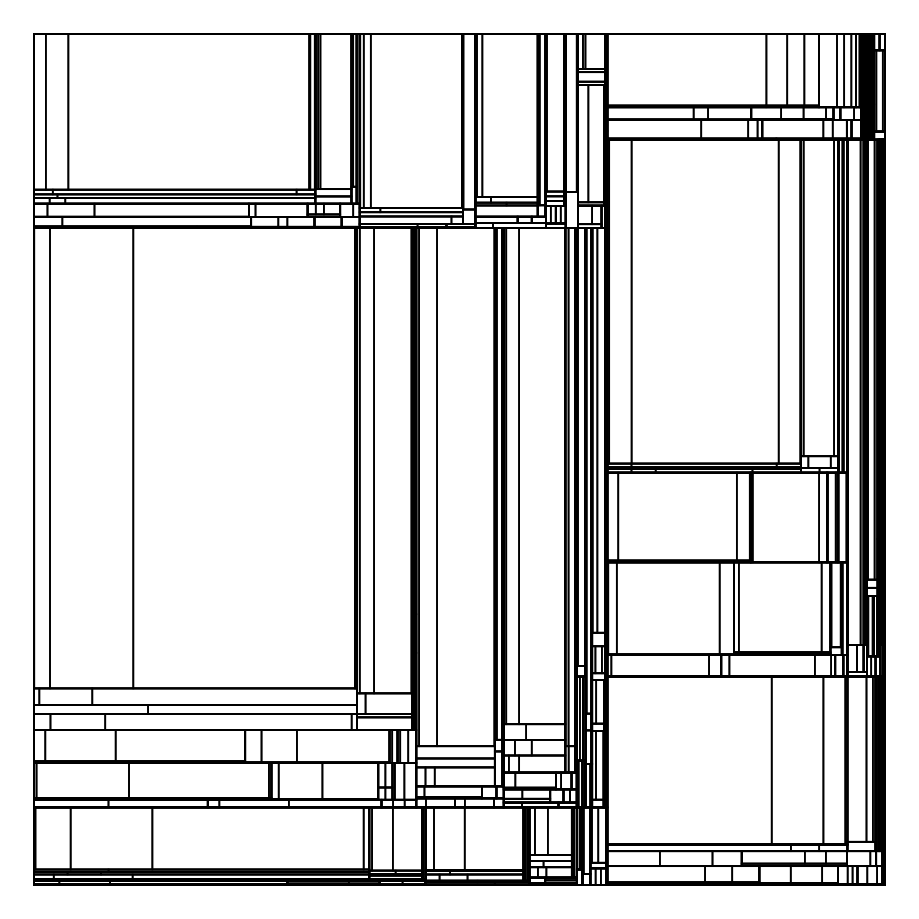
\includegraphics[width=1\linewidth]{../report/figures/tree-treemap-location-type-traffic-regime-intersection-type-road-curvature-road-profile-dedicated-line-road-category}
      \caption{Accidents by all available dimensions.}
    \end{figure}
  \end{minipage}
\end{frame}

\begin{frame}{Visualizations}
  \framesubtitle{Accident Type Treemap}
  \begin{itemize}
    \setlength{\itemsep}{3ex}
    \item identify categories of frequent accidents
    \item by clustering accidents hierarchically
    \item display weighted tree as treemap, graph, or nested list
    \item reorder dimensions
    \item enable/disable partitioning for dimensions
  \end{itemize}
\end{frame}

\begin{frame}{Visualizations}
  \framesubtitle{Interactive Filtering}
  \begin{itemize}
    \setlength{\itemsep}{3ex}
    \item explore differences in groups of similar accidents
    \item select filtered subset of accidents
    \begin{itemize}
      \item select geographic clusters from map
      \item select nodes from treemap
    \end{itemize}
    \item then switch to other visualizations
    \item e.g., \enquote{In curved, sloped roads, when do most accidents occur?}
  \end{itemize}
\end{frame}

\begin{frame}{Demo}
  \centering
  A live demo is deployed at:
  \vspace{2ex}
  \par
  \faIcon{link}
  \enskip
  \footnotesize
  \url{https://heinrichreimer.github.io/france-accidents/}
\end{frame}

\begin{frame}{Related Work}
  \framesubtitle{\textcite{LeLL2020}}
  \citetitle{LeLL2020}
  \begin{itemize}
    \item 1132~accidents in Hanoi~(Vietnam)~2015--2017
    \item severity index~\cite{GeurtsWBV2004}: weighted sum of light, severe, fatal accidents
    \item aggregation per grid (Kernel Density Estimation~\cite{Anderson2009})
    \item map includes street paths
    \item not interactive
  \end{itemize}
  \begin{figure}
    \centering
    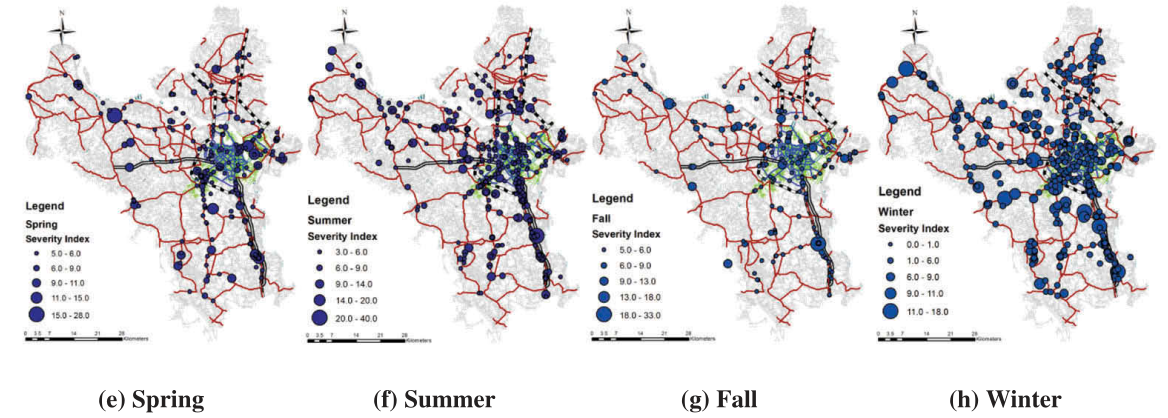
\includegraphics[width=0.8\linewidth]{figures/le2020}
    \caption{Severity index on a map for different seasons.~\cite{LeLL2020}}
  \end{figure}
\end{frame}

\begin{frame}{Related Work}
  \framesubtitle{\textcite{LavravcJTK2008}}
  \citetitle{LavravcJTK2008}
  \begin{itemize}
    \item 453\,451~accident in Slovakia~1995--2005
    \item indicate seasonal influences
    \item two-dimensional heatmap by months and weekdays
    \item greyscale color coding
    \item not interactive
  \end{itemize}
  \begin{figure}
    \centering
    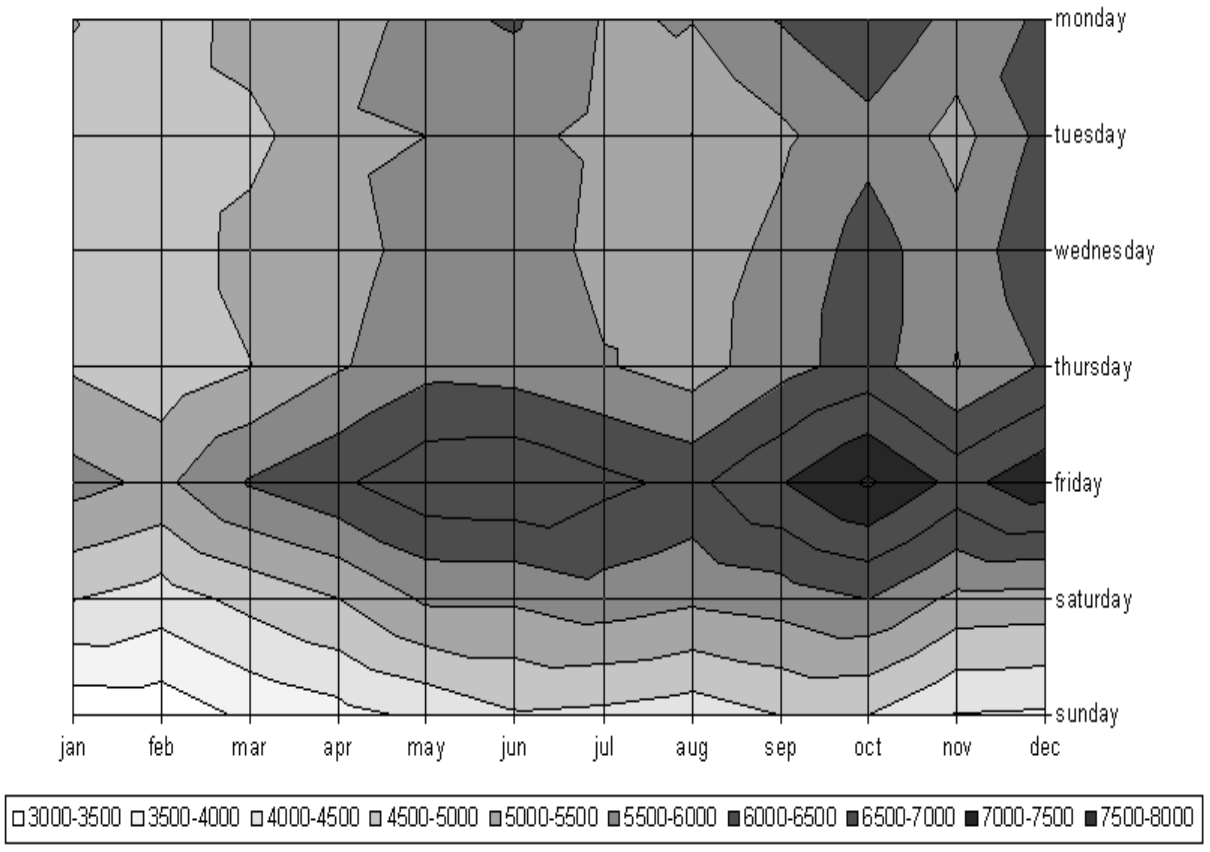
\includegraphics[width=0.4\linewidth]{figures/lavrac2008}
    \caption{Heatmap of accidents for months and weekdays.~\cite{LavravcJTK2008}}
  \end{figure}
\end{frame}

\begin{frame}{Conclusion}
  \begin{itemize}
    \item[\faIcon{github}] \href{https://github.com/heinrichreimer/france-accidents}{\texttt{heinrichreimer/france-accidents}}
    \item three intuitive visualizations
    \begin{itemize}
      \item help citizens to dangerous months or places
      \item support government in targeted education or regulation
      \item let infrastructure planners find problematic/needed infrastructure
    \end{itemize}
    \item men more often involved in accidents
    \item winter slightly safer than summer
  \end{itemize}
  \vspace{1ex}
  \begin{block}{Future Work}
    \begin{itemize}
      \item recursive pattern for time series
      \item improve the map design / other icon designs
      \item more dimensions and filters
      \item use the whole dataset
    \end{itemize}
  \end{block}
  \only<1>{\color{white}}\only<2->{}%
  \thankyou
\end{frame}

\appendix
\section{\appendixname}

\bibliographyframe

\end{document}